\documentclass{article}
\usepackage{hyperref}
\usepackage{fancyhdr}
\usepackage{graphicx}
\usepackage{amsmath}
\usepackage{amssymb}
\usepackage{float}
\usepackage{enumitem}
\usepackage{mathtools}

% if you want to create a new list from scratch
\newlist{alphalist}{enumerate}{1}
% in that case, at least label must be specified using \setlist
\setlist[alphalist,1]{label=\textbf{\alph*.}}

% \graphicspath{{images/}}
\pagestyle{fancy}
\title{EE 271: Final Project Inference Engine on FPGA}
\author{Jay Pankaj Patel}
\date{\today}

\begin{document}
\maketitle
\tableofcontents
\newpage

\section{Building Blocks}
For our inference implementation, I am considering using Convolutional Neural Networks (CNNs). They are an algorithm used to recognize patterns in data. I believe the target data should be handwritten digits from 0--9. Neural networks are built using a collection of neurons organized into layers, each with their own weights and biases. The building blocks of CNNs are the following:
\begin{itemize}
  \item \textbf{Tensor} -- can be thought of as an $n$-dimensional matrix. We need to decide how big to make our tensor. I was considering making it smaller, like three dimensions, because our goal is to perform simple classification.
  \item \textbf{Neuron} -- is a mathematical function that takes multiple inputs and gives a single output.
  \item \textbf{Layer} -- is simply defined as a collection of neurons.
  \item \textbf{Kernel Weights and Biases} -- unique to each neuron and are determined during the training phase of our network. We will train the model on a computer and extract the weights and biases to the FPGA for inference.
  \item \textbf{Differentiable Score Function} -- represented as class scores on the output layer.
\end{itemize}
These are the high-level components needed. Using this knowledge, let’s go over the proposed design.

\section{Design}
Our neural network is going to be as simple as possible because the emphasis of this project will be optimizing the operations required for the model to run. Hence, we are using the "Hello World" equivalent of Machine Learning. Our architecture is as follows. 

\subsection{Architecture}
Our design will take a \textbf{28×28 grayscale image} as input.

After:
\begin{itemize}
  \item A \textbf{convolution layer} will be used to apply 8 kernels to the input, generating \textbf{8 feature maps of size 26×26}, which are then passed to a max-pooling layer.
  \item A \textbf{max-pooling layer} will reduce the \textbf{spatial dimensions} of each feature map from \textbf{26×26 to 13×13}, maintaining 8 feature maps, and will pass the results to the softmax layer.
  \item For training, a \textbf{softmax layer} will process the \textbf{flattened feature maps} and produce \textbf{10 probability values}, each representing the likelihood of the image belonging to one of the 10 classes (digits 0–9).
  \item For the inference and implementation on hardware, a \textbf{hardmax layer} will be used as implementing softmax on hardware is resource intensive and will increase development time.
\end{itemize}

Here is a visual representation of these processes.
\begin{figure}[H]
  \begin{center}
    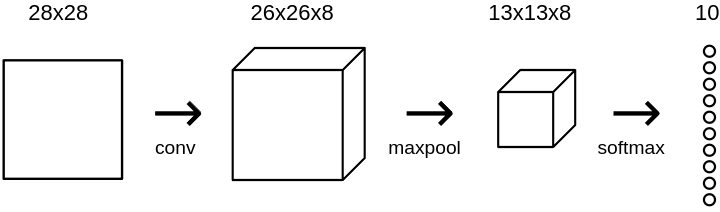
\includegraphics[width=0.95\textwidth]{figures/arch_vis_training}
  \end{center}
  \caption{Visual representation of the CNN layers that will implemented as training in software}\label{fig:cnn_arch}
\end{figure}
\begin{figure}[H]
  \begin{center}
    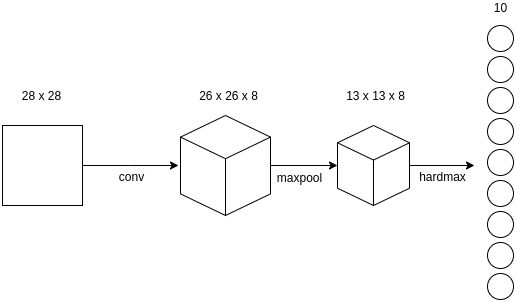
\includegraphics[width=0.95\textwidth]{figures/arch_vis}
  \end{center}
  \caption{Visual representation of the CNN layers that will implemented in hardware}\label{fig:cnn_arch}
\end{figure}
\newpage 
\subsection{Model}
A Python golden model has been created and should be used to validate the FPGA implementation. The Python model is not optimized for hardware, and operations should be adjusted for efficient computation on the FPGA. The model has been pre-trained in Python, and the trained weights and biases will be ported to the FPGA for inference. FPGA-specific design considerations will be discussed after detailing the theory behind each layer.

\subsection{Convolutional Layer Design}
\subsubsection{Background}
\begin{itemize}
  \item \textbf{What is a feature?} \\
    A feature is an individual measurable property that a model uses to make a prediction or classification.
  \item \textbf{What is a feature map?} \\
    A feature map is the output produced when a convolutional kernel extracts relevant features from an input. In this field, the 'filter' is referred to as a \emph{kernel}. Hence, I will be using "kernel" from this point forward.
  \item \textbf{What is convolution?} \\
    Convolution, in a mathematical sense, is an operation performed on two functions that produces a third function. The mathematical operation is defined as the integral of the two functions after one of them is reflected about the y-axis and shifted. Mathematically:
\end{itemize}

\subsection{Equations}
\begin{align*}
  \left( f  * g \right) \left( t \right) &= \int_{-\infty}^{\infty} f \left( \tau \right) g \left( t - \tau \right) \, d\tau
\end{align*}

Graphically:
\begin{figure}[H]
  \begin{center}
    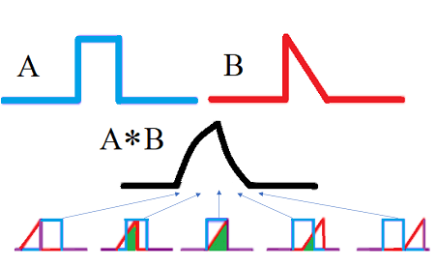
\includegraphics[width=0.5\textwidth]{figures/math_con}
  \end{center}
  \caption{Convolution of two functions A (red) and B (blue) producing a third function describing the overlap (green)}\label{fig:convolution}
\end{figure}

Since we are dealing with discrete systems, convolution is defined using summation instead of an integral:

\begin{align*}
  \left( f * g \right) \left[ n \right] &= \sum_{m = -\infty}^{\infty} f \left[ m\right] g \left[ n-m \right]
\end{align*}

In CNNs, the most computationally expensive operation is the convolution layer. The convolution of the input feature map with the kernel results in an output feature map:

\begin{align*}
  \Aboxed{  y'_j = f \left( \sum_{i \in M_j}^{} x^{l-1}_{i}  * k^l_{ij} + b^l_{j}\right)}
\end{align*}

Where:
\begin{itemize}
  \item \( y^{l}_j \) : Feature map of the \( j \)th convolution kernel result of the \( l  \)th layer.
  \item \( M_{j} \) : Represents the selection of the previous input feature map by the current convolution.
  \item \( x_{i }^{l-1} \): Represents the previous input feature map.
  \item \( k_{ij}^l  \): Represents the \( i  \)th weighting coefficient of the \( j  \)th convolution of the \( l  \)th layer.
  \item \( b^{l }_j \) : Represents the bias parameter of the \( j  \)th convolution kernel of the \( l  \)th layer.
  \item \( f \) : The nonlinear activation function.
\end{itemize}

\subsection{Pooling Layer Design}
\subsubsection{Background}
\begin{itemize}
  \item \textbf{What is pooling?} \\
    Pooling is a technique used to downsample feature maps by aggregating adjacent values.
  \item \textbf{Why pooling?} \\
    Neighboring pixels in images tend to have similar values, leading to redundant information. Pooling reduces this redundancy while retaining important features.
  \item \textbf{How is pooling done?} \\
    Pooling is implemented using a max, min, or average value comparison over a small region.
\end{itemize}

\subsection{Pooling Equation}
A 3×3 convolution computes each output pixel using a weighted sum of a 3×3 region from the input:

\begin{align*}
  \Aboxed{ Y(i, j) &= \sum_{m=0}^{2} \sum_{n=0}^{2} X(i+m, j+n) \cdot W(m, n)}
\end{align*}

Where:
\begin{itemize}
  \item \( X(i, j) \) is the input feature map (28×28).
  \item \( W(m, n) \) is the 3×3 convolution kernel (filter).
  \item \( Y(i, j) \) is the output feature map after convolution.
\end{itemize}

Valid padding means no padding is added, so the output size is:

\[
(28-3+1) \times (28-3+1) = 26 \times 26
\]
And we repeat this 8 times because we have 8 kernels. Hence our final output will be 26 x 26 x 8.

\subsection{Softmax Layer Design}
\subsubsection{Background} 
\begin{itemize}
  \item \textbf{What is an activation function?}
    An activation function allows our model to achieve non-linearity as most things in real life are not a linear equation. By doing so, it allows our model to achieve higher accuracies.
  \item \textbf{What is softmax?} 
    Softmax is an activation function that converts an arbitrary set of numbers into a probability distribution. 
  \item \textbf{Why Softmax?} 
      Softmax is useful when you have a multi-class model as we do here, (0-9 are different classes). 
\end{itemize}

\subsection{Softmax Equation} 
Mathematically, given an input vector \( x = [x_1, x_2, ..., x_n] \), the Softmax function is defined as:

\begin{align*}
  \Aboxed{s(x_i) = \frac{e^{x_i}}{\sum_{j=1}^{n} e^{x_j}}}
\end{align*}
where:
\begin{itemize}
    \item \( x_i \) represents the raw input (logit) for class \( i \).
    \item \( e^{x_i} \) represents exponentiation of the input values.
    \item The denominator is the \textbf{sum of exponentials} over all input values.
    \item The function ensures that all outputs sum to 1.
\end{itemize}
\subsubsection{Sample Calculation} 
\begin{enumerate}
    \item Compute exponentials:
    \[
    e^{-1} = 0.368, \quad e^0 = 1, \quad e^3 = 20.09 \\
    \quad e^5 = 148.41
    \]

    \item Compute denominator (sum of exponentials):
    \[
    0.368 + 1 + 20.09 + 148.41 = 169.87
    \]

    \item Compute Softmax probabilities:
    \begin{align*}
      s(-1) &= \frac{0.368}{169.87} = 0.002\\ 
      s(0) &= \frac{1}{169.87} = 0.006\\ 
      s(3) &= \frac{20.09}{169.87} = 0.118\\ 
      s(5) &= \frac{148.41}{169.87} = 0.874
    \end{align*}
\end{enumerate}

Thus, the final probability distribution is:
\[
[0.002, 0.006, 0.118, 0.874]
\]

This means the model is \textbf{87.4\% confident in class 5} and assigns lower probabilities to other classes.

\subsection{Hardmax Layer Design}
\subsubsection{Background} 
\begin{itemize}
  \item \textbf{What is hardmax?}  
    Hardmax is a function that converts a set of values into a one-hot encoded vector, where only the index with the highest value is set to 1 and all others are set to 0.
  \item \textbf{Why Hardmax?}  
    Hardmax is useful during inference when we want to make a final decision and select the most likely class. It is deterministic and discrete, which makes it appropriate for classification output.
\end{itemize}

\subsection{Hardmax Equation}
Given an input vector \( x = [x_1, x_2, ..., x_n] \), the Hardmax function outputs a vector \( h = [h_1, h_2, ..., h_n] \), where:

\[
h_i =
\begin{cases}
1 & \text{if } i = \arg\max_j x_j \\
0 & \text{otherwise}
\end{cases}
\]

\noindent where:
\begin{itemize}
    \item \( x_i \) represents the raw input (logit) for class \( i \).
    \item \( \arg\max_j x_j \) returns the index of the maximum value in the input vector.
    \item The result is a one-hot vector with a 1 at the index of the largest value.
\end{itemize}

\subsubsection{Sample Calculation} 
\begin{enumerate}
    \item Input vector:
    \[
    x = [-1,\ 0,\ 3,\ 5]
    \]

    \item Find index of maximum value:
    \[
    \arg\max(x) = 3 \quad \text{(since } x_4 = 5 \text{ is largest)}
    \]

    \item Convert to one-hot encoding:
    \[
    h = [0,\ 0,\ 0,\ 1]
    \]
\end{enumerate}

\noindent Thus, the final hardmax output is:
\[
[0,\ 0,\ 0,\ 1]
\]

\noindent This means the model predicts class 3 with full confidence and disregards the other classes completely.





\end{document}
